\documentclass[11pt]{article}
\usepackage[textwidth=18.0cm, textheight=23.0cm, top=2.0cm]{geometry}
\usepackage{pst-all}
\usepackage{amssymb}
\usepackage{tikz}
\usepackage{underscore}\begin{document}
\pagestyle{empty}


ClassName: \underline{\textbf{Class_10.2bp-21}}
\par
BinSize: \underline{\textbf{100 × 100}}
\par
ReduceSize: \underline{\textbf{100 × 100}}
\par
TypeNum: \underline{\textbf{59}}
\par
Num: \underline{\textbf{60}}
\par
OutS: \underline{\textbf{120000}}
\par
InS: \underline{\textbf{108960}}
\par
Rate: \underline{\textbf{0.908}}
\par
UB: \underline{\textbf{12}}
\par
LB0: \underline{\textbf{12}}
\par
LB: \underline{\textbf{12}}
\par
LBWithCut: \underline{\textbf{12}}
\par
NodeCut: \underline{\textbf{0}}
\par
ExtendedNodeCnt: \underline{\textbf{1}}
\par
GenNodeCnt: \underline{\textbf{1}}
\par
PrimalNode: \underline{\textbf{0}}
\par
ColumnCount: \underline{\textbf{12}}
\par
TotalCutCount: \underline{\textbf{0}}
\par
RootCutCount: \underline{\textbf{0}}
\par
LPSolverCnt: \underline{\textbf{1}}
\par
PricingSolverCnt: \underline{\textbf{0}}
\par
BranchAndBoundNum: \underline{\textbf{1}}
\par
isOpt: \underline{\textbf{true}}
\par
TimeOnInitSolution: \underline{\textbf{600.000 s}}
\par
TimeOnPrimal: \underline{\textbf{0.000 s}}
\par
TimeOnPricing: \underline{\textbf{0.000 s}}
\par
TimeOnRmp: \underline{\textbf{0.094 s}}
\par
TotalTime: \underline{\textbf{600.360 s}}
\par
\newpage


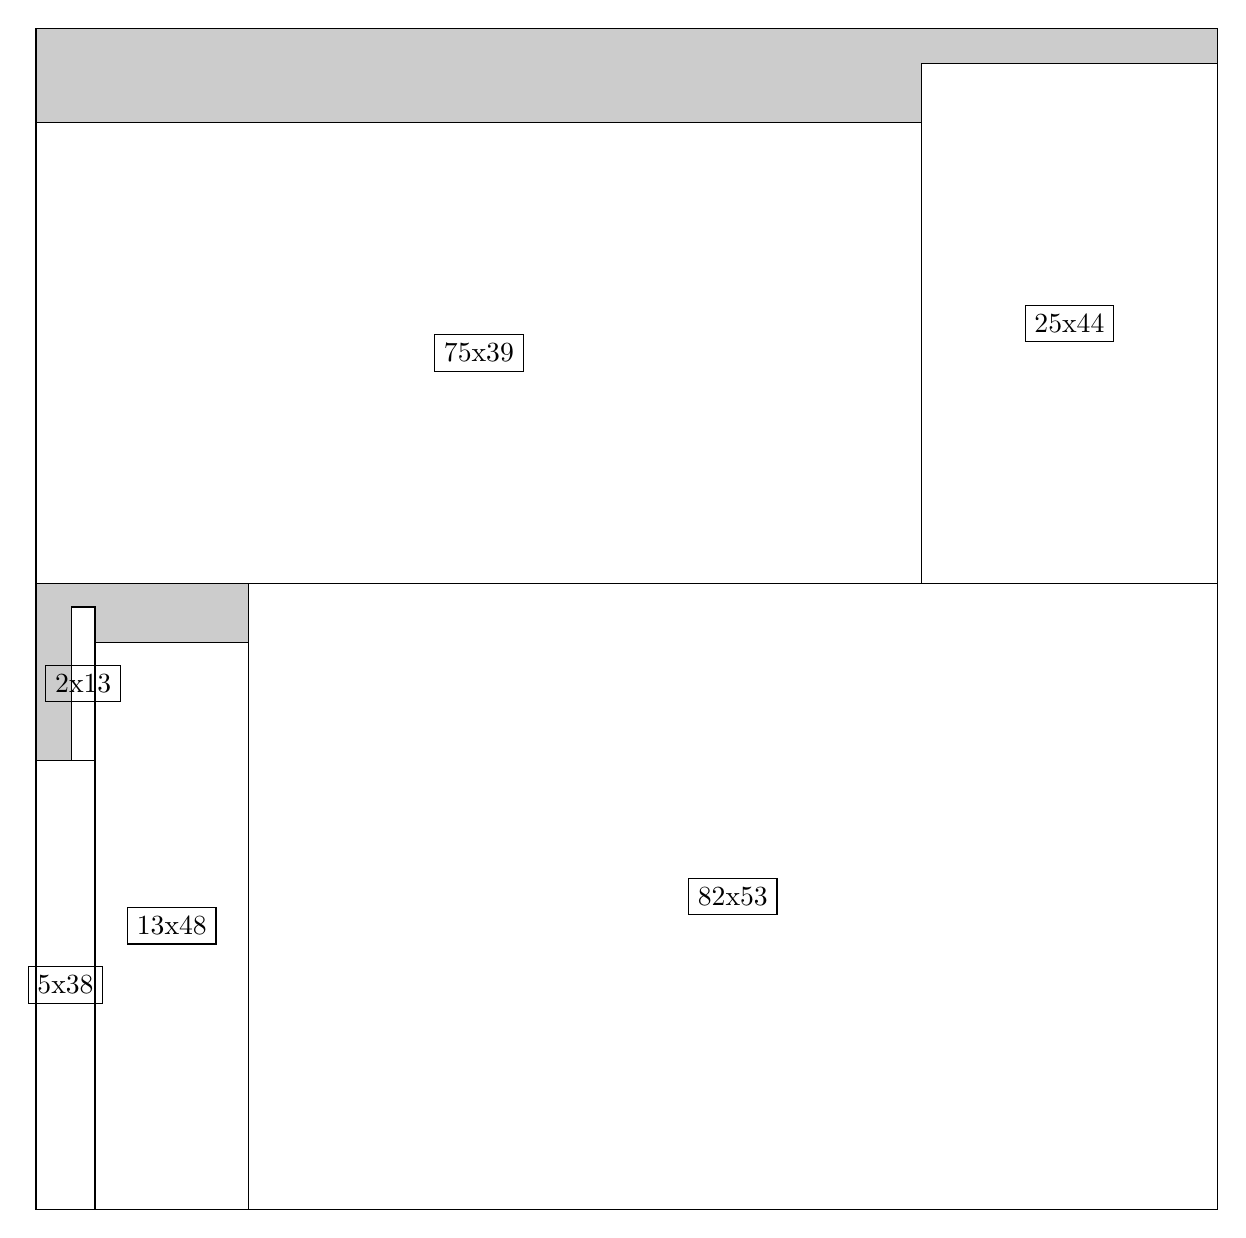
\begin{tikzpicture}[shorten >=1pt,scale=1.0,every node/.style={scale=1.0},->]
\tikzstyle{vertex}=[circle,fill=black!25,minimum size=14pt,inner sep=0pt]
\filldraw[fill=gray!40!white, draw=black] (0,0) rectangle (15.0,15.0);
\foreach \name/\x/\y/\w/\h in {82x53/2.6999999999999997/0.0/12.299999999999999/7.949999999999999,13x48/0.75/0.0/1.95/7.199999999999999,5x38/0.0/0.0/0.75/5.7,2x13/0.44999999999999996/5.7/0.3/1.95,25x44/11.25/7.949999999999999/3.75/6.6,75x39/0.0/7.949999999999999/11.25/5.85}
\filldraw[fill=white!40!white, draw=black] (\x,\y) rectangle node[draw] (\name) {\name} ++(\w,\h);
\end{tikzpicture}


w =82 , h =53 , x =18 , y =0 , v =4346
\par
w =13 , h =48 , x =5 , y =0 , v =624
\par
w =5 , h =38 , x =0 , y =0 , v =190
\par
w =2 , h =13 , x =3 , y =38 , v =26
\par
w =25 , h =44 , x =75 , y =53 , v =1100
\par
w =75 , h =39 , x =0 , y =53 , v =2925
\par
\newpage


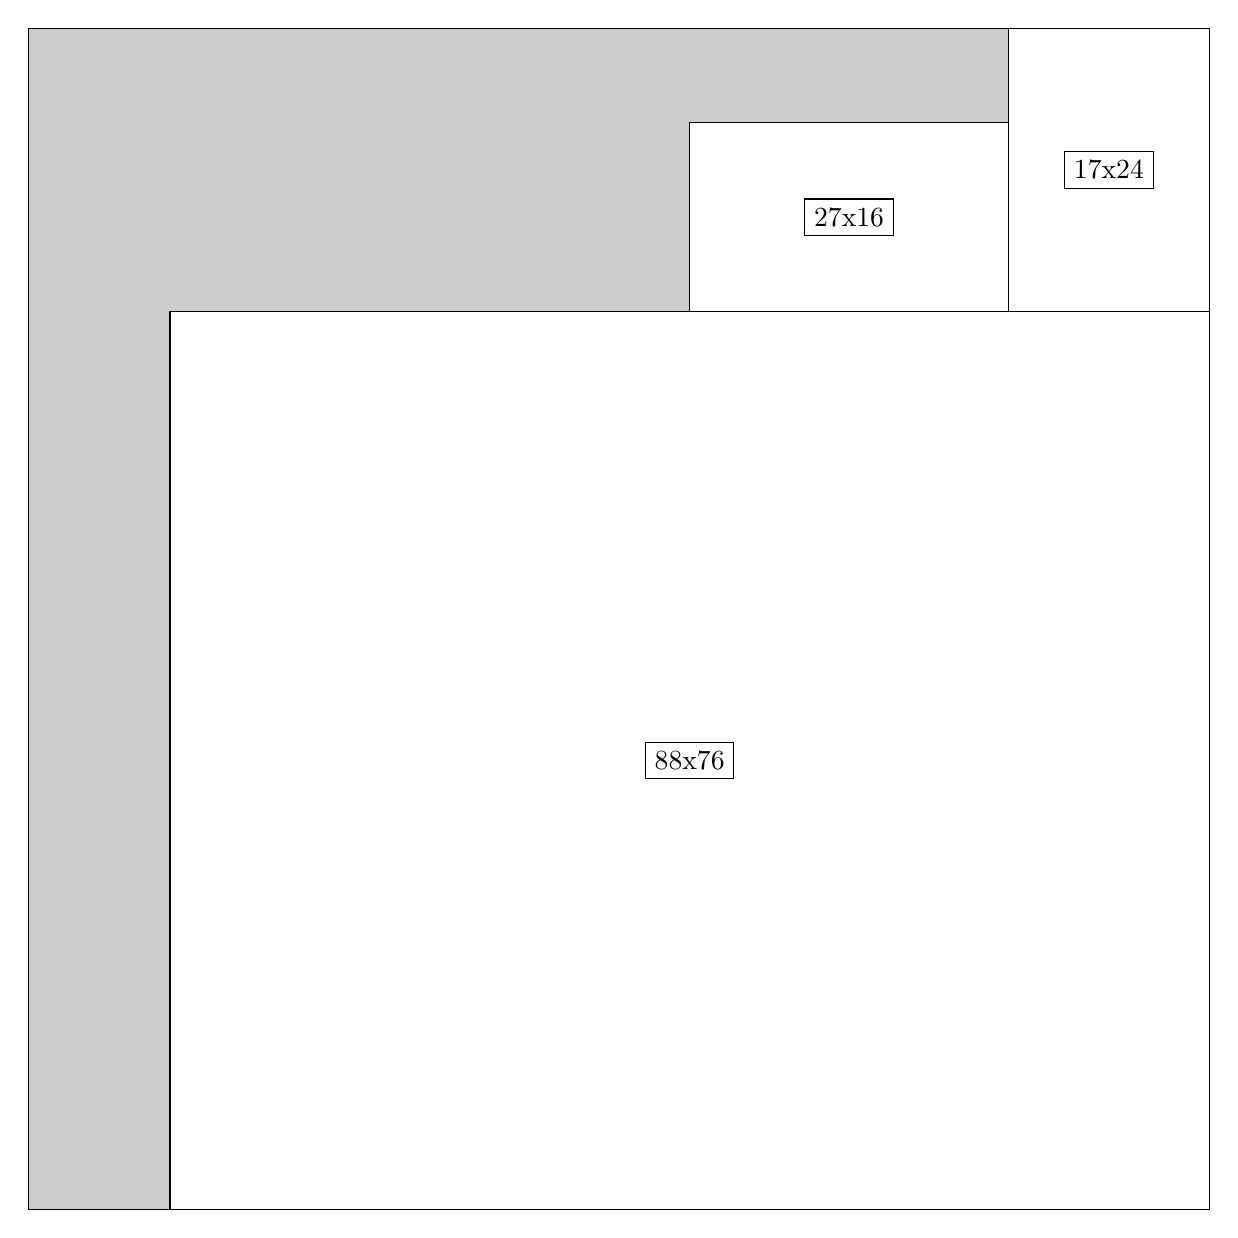
\begin{tikzpicture}[shorten >=1pt,scale=1.0,every node/.style={scale=1.0},->]
\tikzstyle{vertex}=[circle,fill=black!25,minimum size=14pt,inner sep=0pt]
\filldraw[fill=gray!40!white, draw=black] (0,0) rectangle (15.0,15.0);
\foreach \name/\x/\y/\w/\h in {88x76/1.7999999999999998/0.0/13.2/11.4,17x24/12.45/11.4/2.55/3.5999999999999996,27x16/8.4/11.4/4.05/2.4}
\filldraw[fill=white!40!white, draw=black] (\x,\y) rectangle node[draw] (\name) {\name} ++(\w,\h);
\end{tikzpicture}


w =88 , h =76 , x =12 , y =0 , v =6688
\par
w =17 , h =24 , x =83 , y =76 , v =408
\par
w =27 , h =16 , x =56 , y =76 , v =432
\par
\newpage


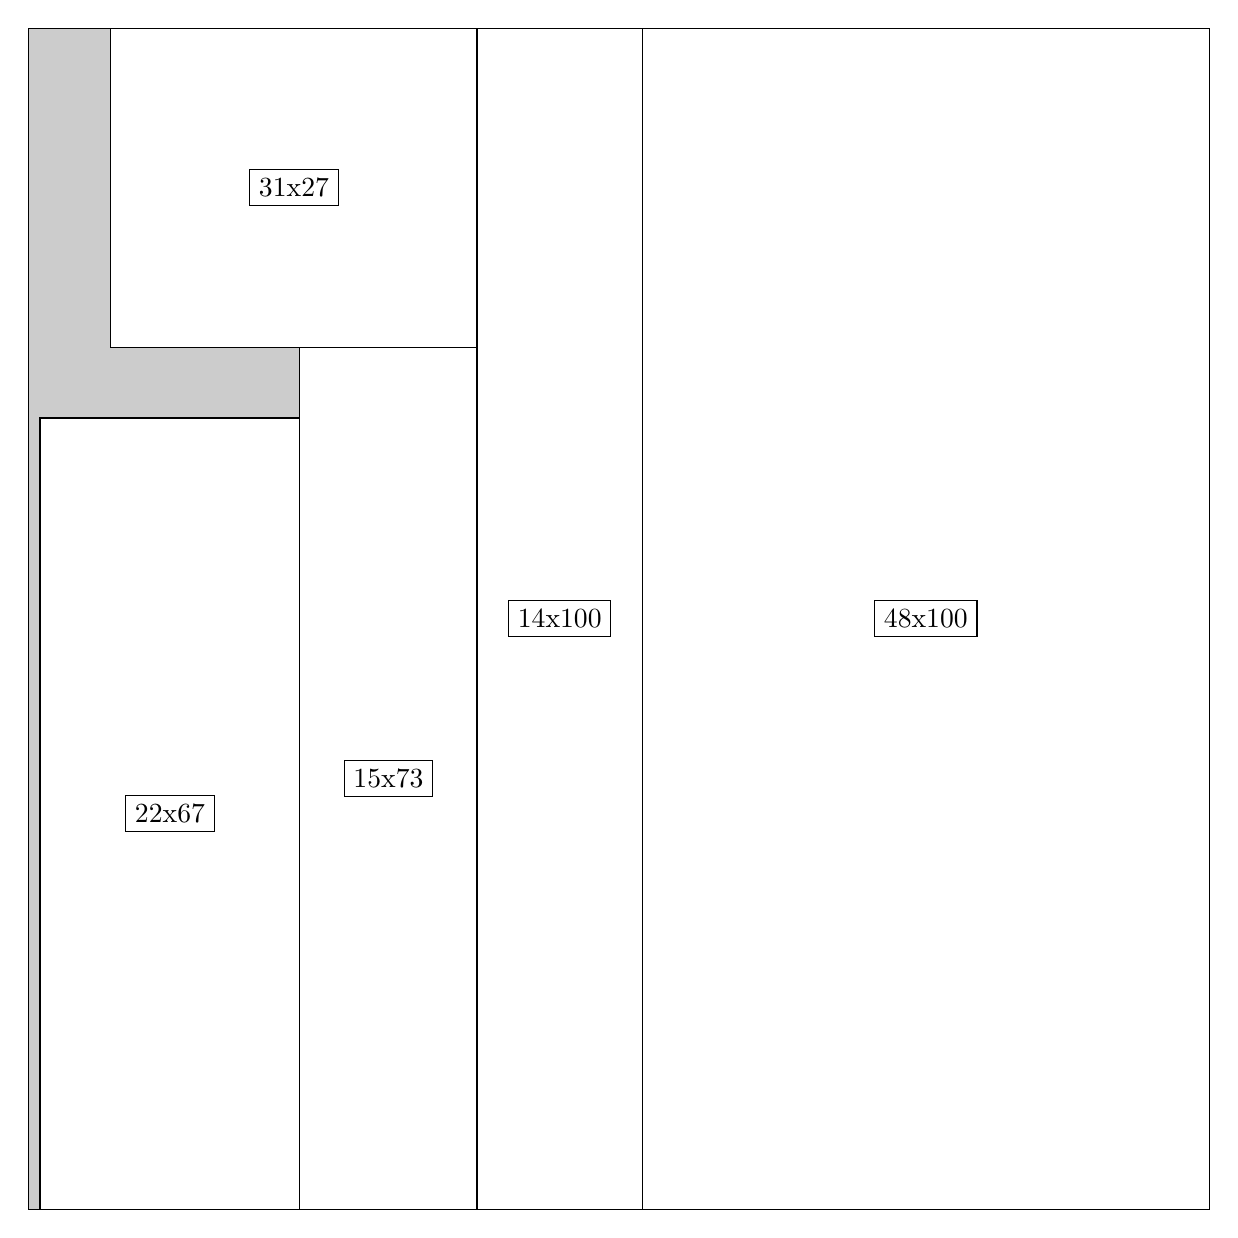
\begin{tikzpicture}[shorten >=1pt,scale=1.0,every node/.style={scale=1.0},->]
\tikzstyle{vertex}=[circle,fill=black!25,minimum size=14pt,inner sep=0pt]
\filldraw[fill=gray!40!white, draw=black] (0,0) rectangle (15.0,15.0);
\foreach \name/\x/\y/\w/\h in {48x100/7.8/0.0/7.199999999999999/15.0,14x100/5.7/0.0/2.1/15.0,15x73/3.4499999999999997/0.0/2.25/10.95,22x67/0.15/0.0/3.3/10.049999999999999,31x27/1.05/10.95/4.6499999999999995/4.05}
\filldraw[fill=white!40!white, draw=black] (\x,\y) rectangle node[draw] (\name) {\name} ++(\w,\h);
\end{tikzpicture}


w =48 , h =100 , x =52 , y =0 , v =4800
\par
w =14 , h =100 , x =38 , y =0 , v =1400
\par
w =15 , h =73 , x =23 , y =0 , v =1095
\par
w =22 , h =67 , x =1 , y =0 , v =1474
\par
w =31 , h =27 , x =7 , y =73 , v =837
\par
\newpage


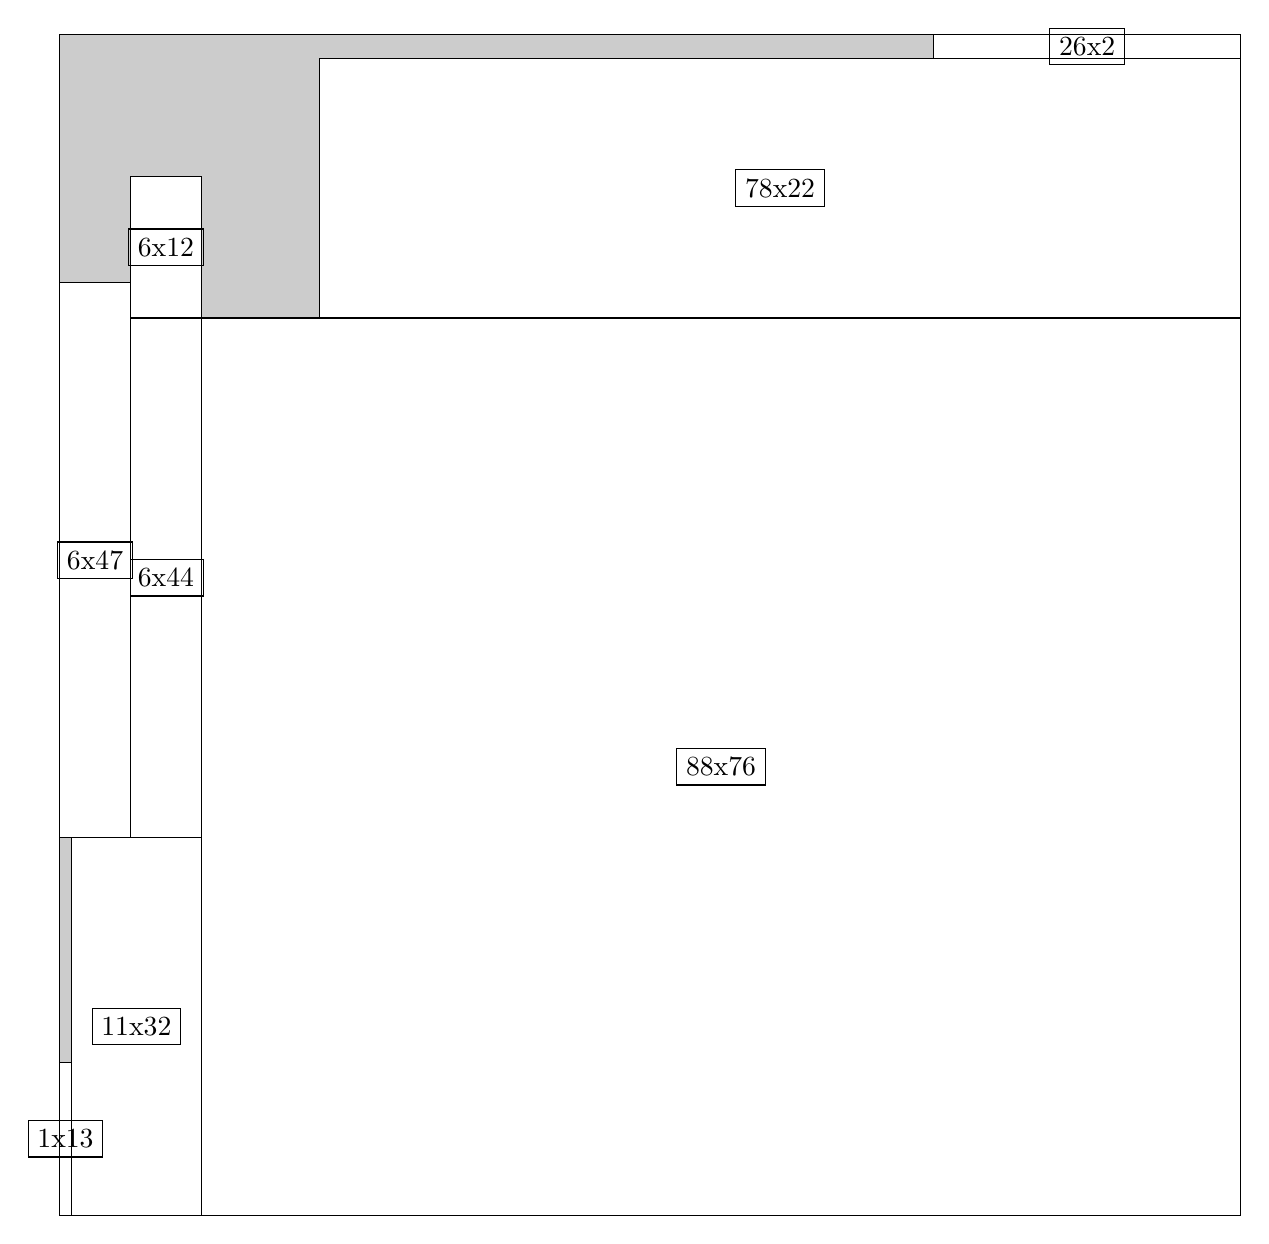
\begin{tikzpicture}[shorten >=1pt,scale=1.0,every node/.style={scale=1.0},->]
\tikzstyle{vertex}=[circle,fill=black!25,minimum size=14pt,inner sep=0pt]
\filldraw[fill=gray!40!white, draw=black] (0,0) rectangle (15.0,15.0);
\foreach \name/\x/\y/\w/\h in {88x76/1.7999999999999998/0.0/13.2/11.4,78x22/3.3/11.4/11.7/3.3,26x2/11.1/14.7/3.9/0.3,11x32/0.15/0.0/1.65/4.8,1x13/0.0/0.0/0.15/1.95,6x44/0.8999999999999999/4.8/0.8999999999999999/6.6,6x12/0.8999999999999999/11.4/0.8999999999999999/1.7999999999999998,6x47/0.0/4.8/0.8999999999999999/7.05}
\filldraw[fill=white!40!white, draw=black] (\x,\y) rectangle node[draw] (\name) {\name} ++(\w,\h);
\end{tikzpicture}


w =88 , h =76 , x =12 , y =0 , v =6688
\par
w =78 , h =22 , x =22 , y =76 , v =1716
\par
w =26 , h =2 , x =74 , y =98 , v =52
\par
w =11 , h =32 , x =1 , y =0 , v =352
\par
w =1 , h =13 , x =0 , y =0 , v =13
\par
w =6 , h =44 , x =6 , y =32 , v =264
\par
w =6 , h =12 , x =6 , y =76 , v =72
\par
w =6 , h =47 , x =0 , y =32 , v =282
\par
\newpage


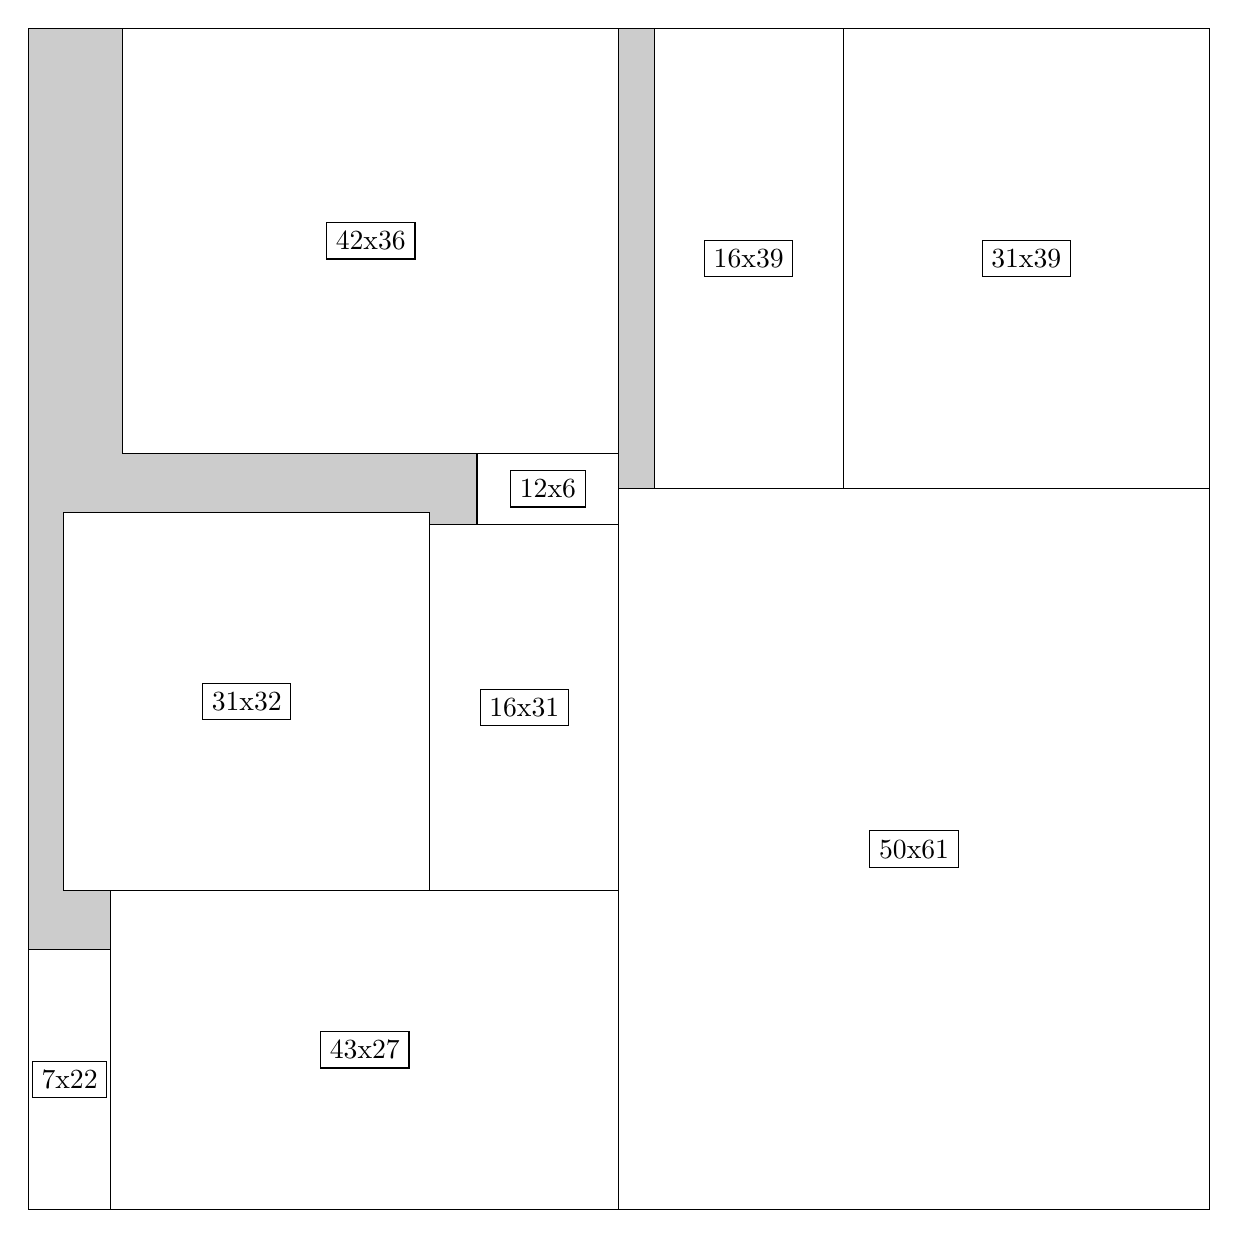
\begin{tikzpicture}[shorten >=1pt,scale=1.0,every node/.style={scale=1.0},->]
\tikzstyle{vertex}=[circle,fill=black!25,minimum size=14pt,inner sep=0pt]
\filldraw[fill=gray!40!white, draw=black] (0,0) rectangle (15.0,15.0);
\foreach \name/\x/\y/\w/\h in {50x61/7.5/0.0/7.5/9.15,31x39/10.35/9.15/4.6499999999999995/5.85,16x39/7.949999999999999/9.15/2.4/5.85,43x27/1.05/0.0/6.45/4.05,7x22/0.0/0.0/1.05/3.3,16x31/5.1/4.05/2.4/4.6499999999999995,12x6/5.7/8.7/1.7999999999999998/0.8999999999999999,31x32/0.44999999999999996/4.05/4.6499999999999995/4.8,42x36/1.2/9.6/6.3/5.3999999999999995}
\filldraw[fill=white!40!white, draw=black] (\x,\y) rectangle node[draw] (\name) {\name} ++(\w,\h);
\end{tikzpicture}


w =50 , h =61 , x =50 , y =0 , v =3050
\par
w =31 , h =39 , x =69 , y =61 , v =1209
\par
w =16 , h =39 , x =53 , y =61 , v =624
\par
w =43 , h =27 , x =7 , y =0 , v =1161
\par
w =7 , h =22 , x =0 , y =0 , v =154
\par
w =16 , h =31 , x =34 , y =27 , v =496
\par
w =12 , h =6 , x =38 , y =58 , v =72
\par
w =31 , h =32 , x =3 , y =27 , v =992
\par
w =42 , h =36 , x =8 , y =64 , v =1512
\par
\newpage


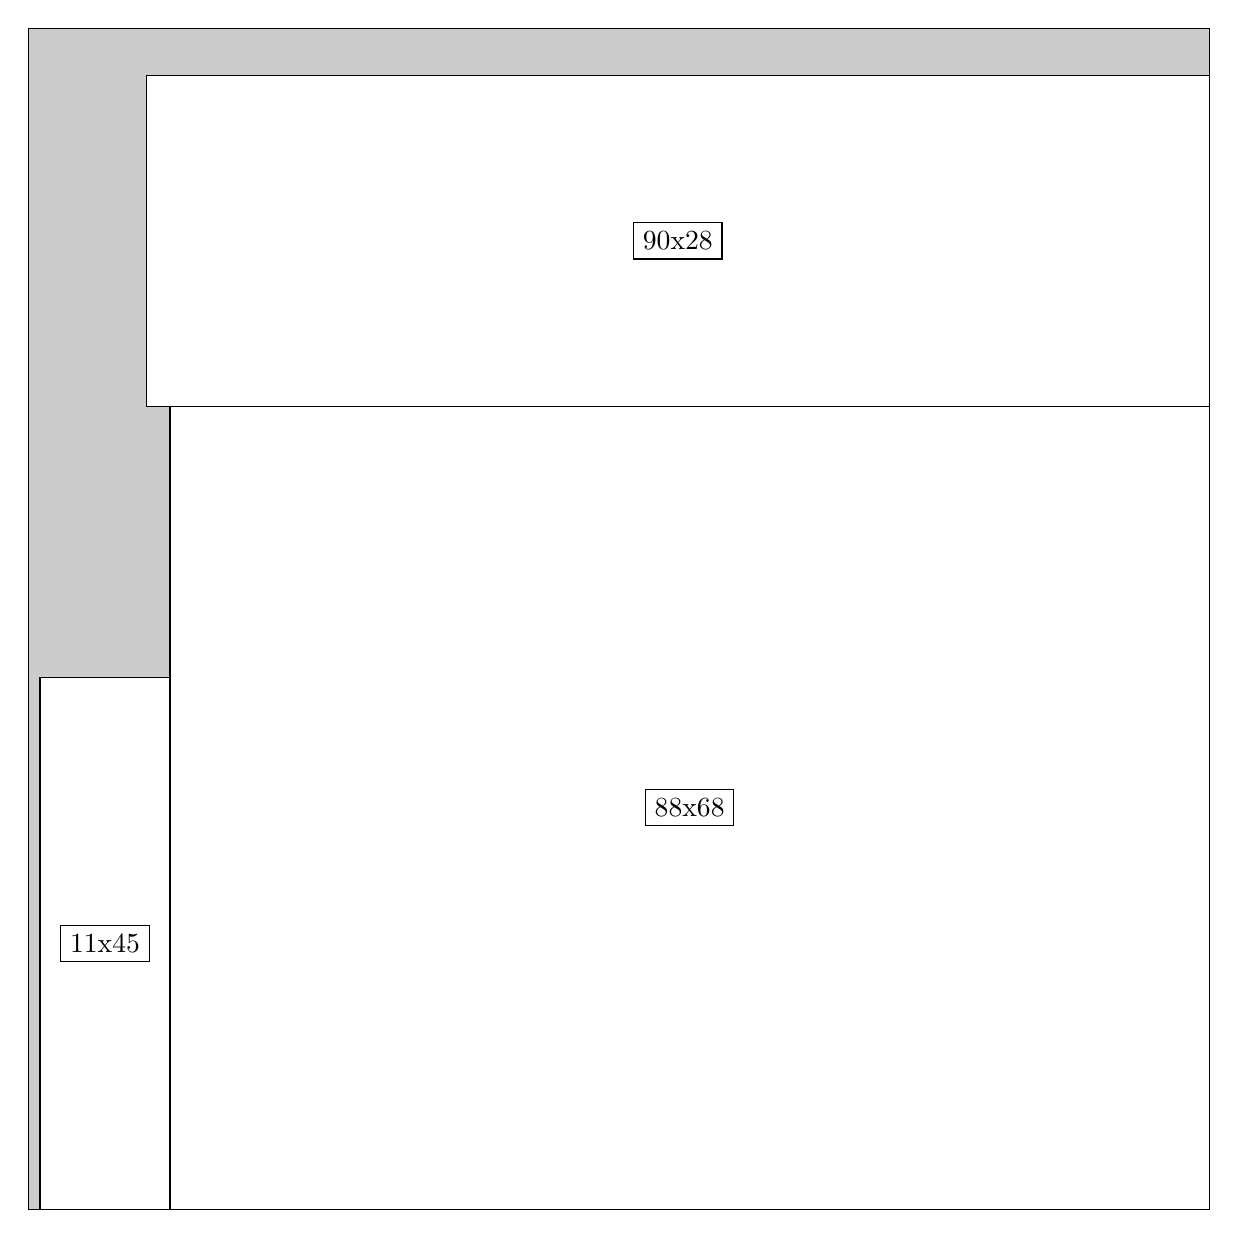
\begin{tikzpicture}[shorten >=1pt,scale=1.0,every node/.style={scale=1.0},->]
\tikzstyle{vertex}=[circle,fill=black!25,minimum size=14pt,inner sep=0pt]
\filldraw[fill=gray!40!white, draw=black] (0,0) rectangle (15.0,15.0);
\foreach \name/\x/\y/\w/\h in {88x68/1.7999999999999998/0.0/13.2/10.2,11x45/0.15/0.0/1.65/6.75,90x28/1.5/10.2/13.5/4.2}
\filldraw[fill=white!40!white, draw=black] (\x,\y) rectangle node[draw] (\name) {\name} ++(\w,\h);
\end{tikzpicture}


w =88 , h =68 , x =12 , y =0 , v =5984
\par
w =11 , h =45 , x =1 , y =0 , v =495
\par
w =90 , h =28 , x =10 , y =68 , v =2520
\par
\newpage


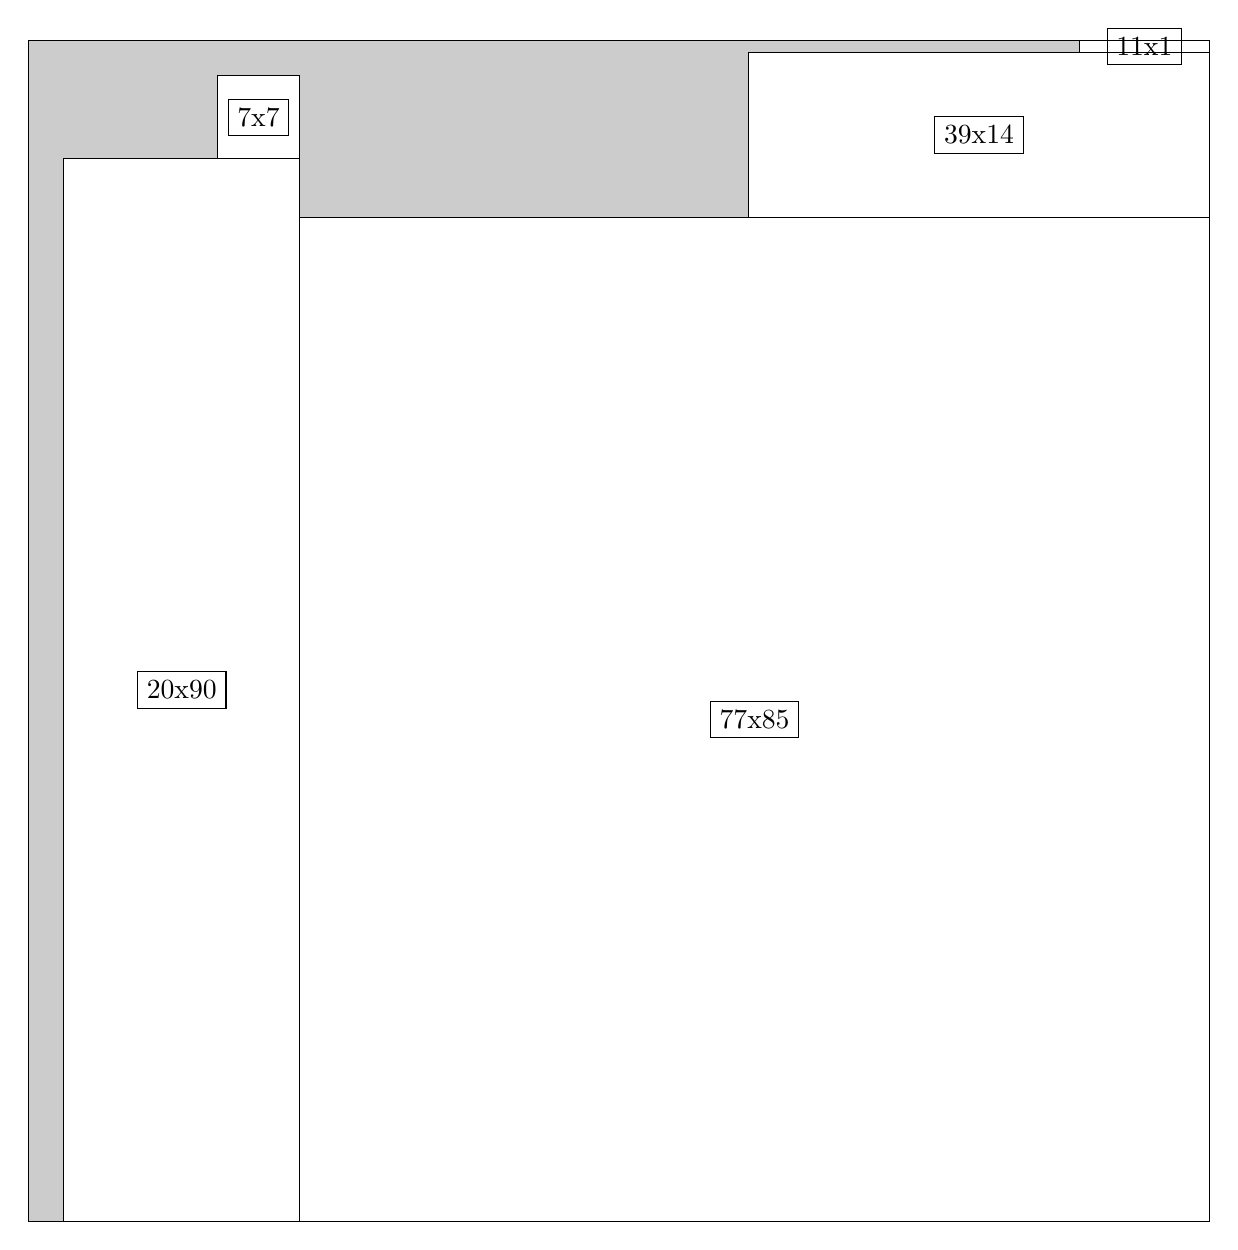
\begin{tikzpicture}[shorten >=1pt,scale=1.0,every node/.style={scale=1.0},->]
\tikzstyle{vertex}=[circle,fill=black!25,minimum size=14pt,inner sep=0pt]
\filldraw[fill=gray!40!white, draw=black] (0,0) rectangle (15.0,15.0);
\foreach \name/\x/\y/\w/\h in {77x85/3.4499999999999997/0.0/11.549999999999999/12.75,39x14/9.15/12.75/5.85/2.1,11x1/13.35/14.85/1.65/0.15,20x90/0.44999999999999996/0.0/3.0/13.5,7x7/2.4/13.5/1.05/1.05}
\filldraw[fill=white!40!white, draw=black] (\x,\y) rectangle node[draw] (\name) {\name} ++(\w,\h);
\end{tikzpicture}


w =77 , h =85 , x =23 , y =0 , v =6545
\par
w =39 , h =14 , x =61 , y =85 , v =546
\par
w =11 , h =1 , x =89 , y =99 , v =11
\par
w =20 , h =90 , x =3 , y =0 , v =1800
\par
w =7 , h =7 , x =16 , y =90 , v =49
\par
\newpage


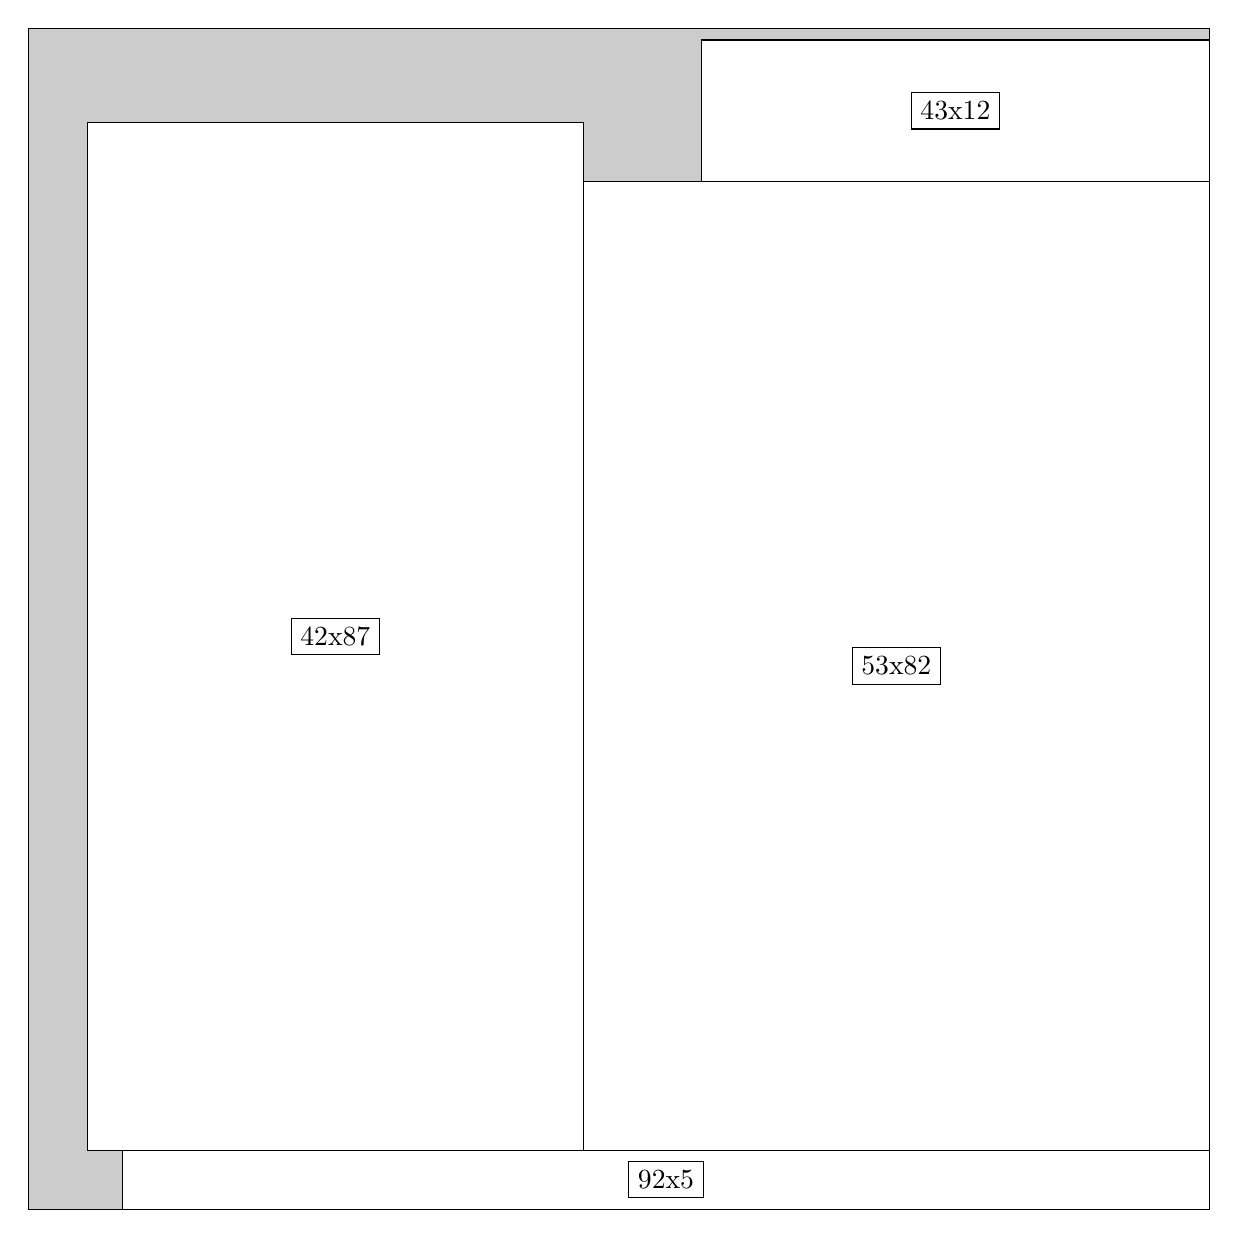
\begin{tikzpicture}[shorten >=1pt,scale=1.0,every node/.style={scale=1.0},->]
\tikzstyle{vertex}=[circle,fill=black!25,minimum size=14pt,inner sep=0pt]
\filldraw[fill=gray!40!white, draw=black] (0,0) rectangle (15.0,15.0);
\foreach \name/\x/\y/\w/\h in {92x5/1.2/0.0/13.799999999999999/0.75,53x82/7.05/0.75/7.949999999999999/12.299999999999999,43x12/8.549999999999999/13.049999999999999/6.45/1.7999999999999998,42x87/0.75/0.75/6.3/13.049999999999999}
\filldraw[fill=white!40!white, draw=black] (\x,\y) rectangle node[draw] (\name) {\name} ++(\w,\h);
\end{tikzpicture}


w =92 , h =5 , x =8 , y =0 , v =460
\par
w =53 , h =82 , x =47 , y =5 , v =4346
\par
w =43 , h =12 , x =57 , y =87 , v =516
\par
w =42 , h =87 , x =5 , y =5 , v =3654
\par
\newpage


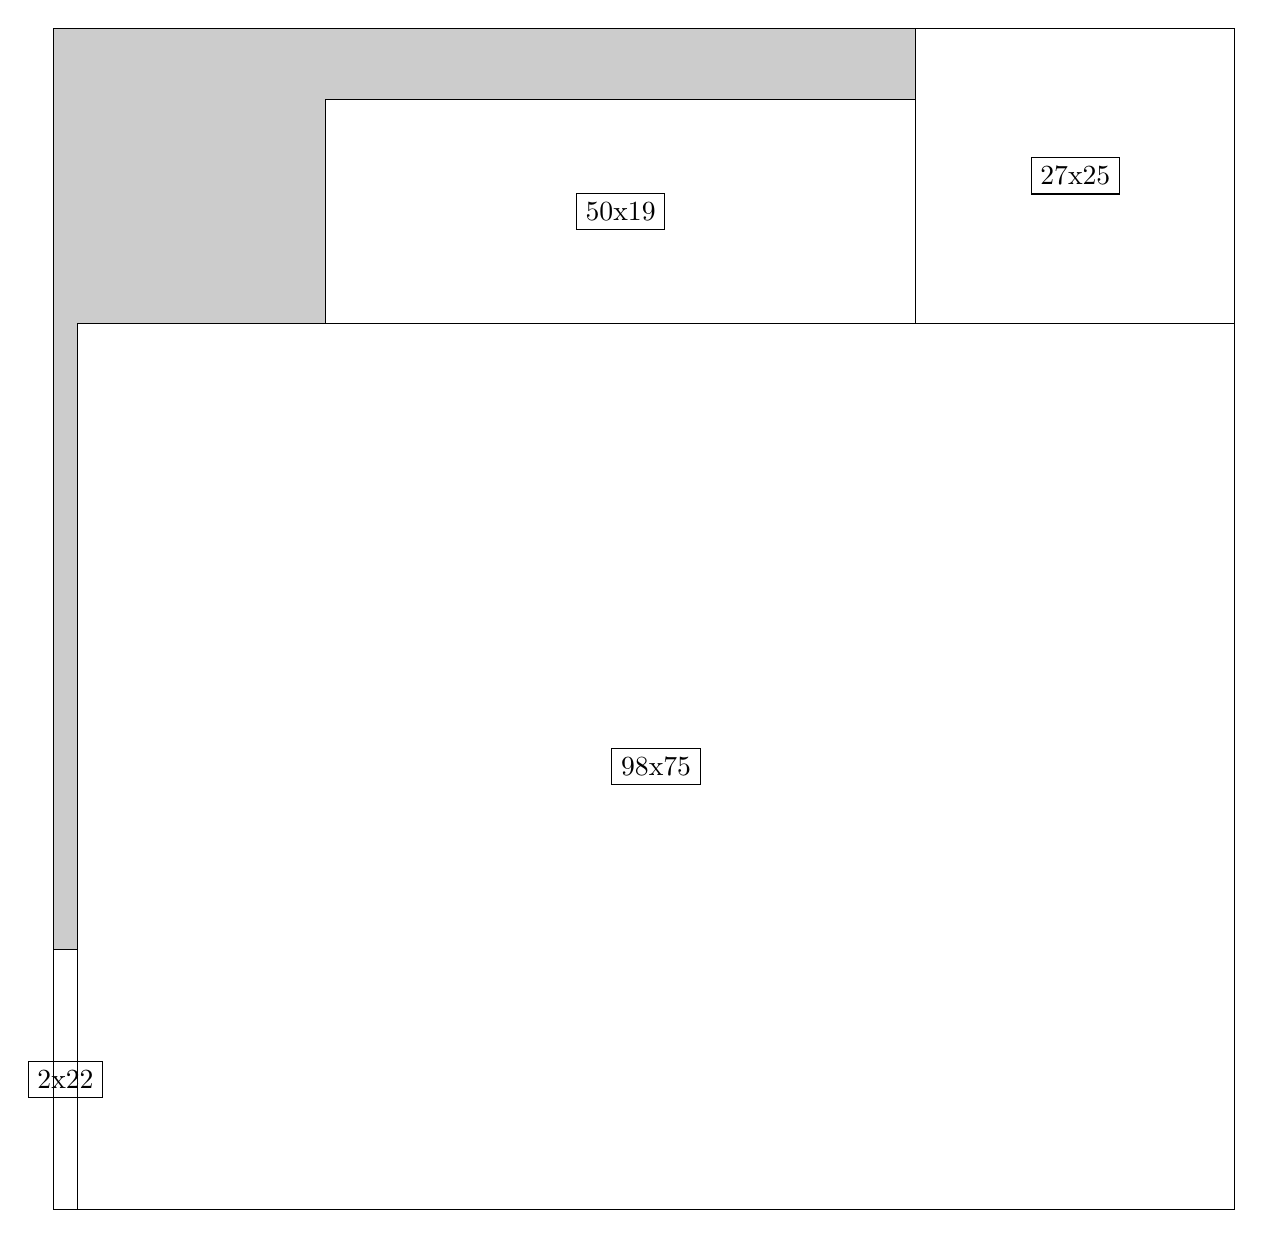
\begin{tikzpicture}[shorten >=1pt,scale=1.0,every node/.style={scale=1.0},->]
\tikzstyle{vertex}=[circle,fill=black!25,minimum size=14pt,inner sep=0pt]
\filldraw[fill=gray!40!white, draw=black] (0,0) rectangle (15.0,15.0);
\foreach \name/\x/\y/\w/\h in {98x75/0.3/0.0/14.7/11.25,2x22/0.0/0.0/0.3/3.3,27x25/10.95/11.25/4.05/3.75,50x19/3.4499999999999997/11.25/7.5/2.85}
\filldraw[fill=white!40!white, draw=black] (\x,\y) rectangle node[draw] (\name) {\name} ++(\w,\h);
\end{tikzpicture}


w =98 , h =75 , x =2 , y =0 , v =7350
\par
w =2 , h =22 , x =0 , y =0 , v =44
\par
w =27 , h =25 , x =73 , y =75 , v =675
\par
w =50 , h =19 , x =23 , y =75 , v =950
\par
\newpage



\begin{tikzpicture}[shorten >=1pt,scale=1.0,every node/.style={scale=1.0},->]
\tikzstyle{vertex}=[circle,fill=black!25,minimum size=14pt,inner sep=0pt]
\filldraw[fill=gray!40!white, draw=black] (0,0) rectangle (15.0,15.0);
\foreach \name/\x/\y/\w/\h in {98x97/0.3/0.0/14.7/14.549999999999999}
\filldraw[fill=white!40!white, draw=black] (\x,\y) rectangle node[draw] (\name) {\name} ++(\w,\h);
\end{tikzpicture}


w =98 , h =97 , x =2 , y =0 , v =9506
\par
\newpage


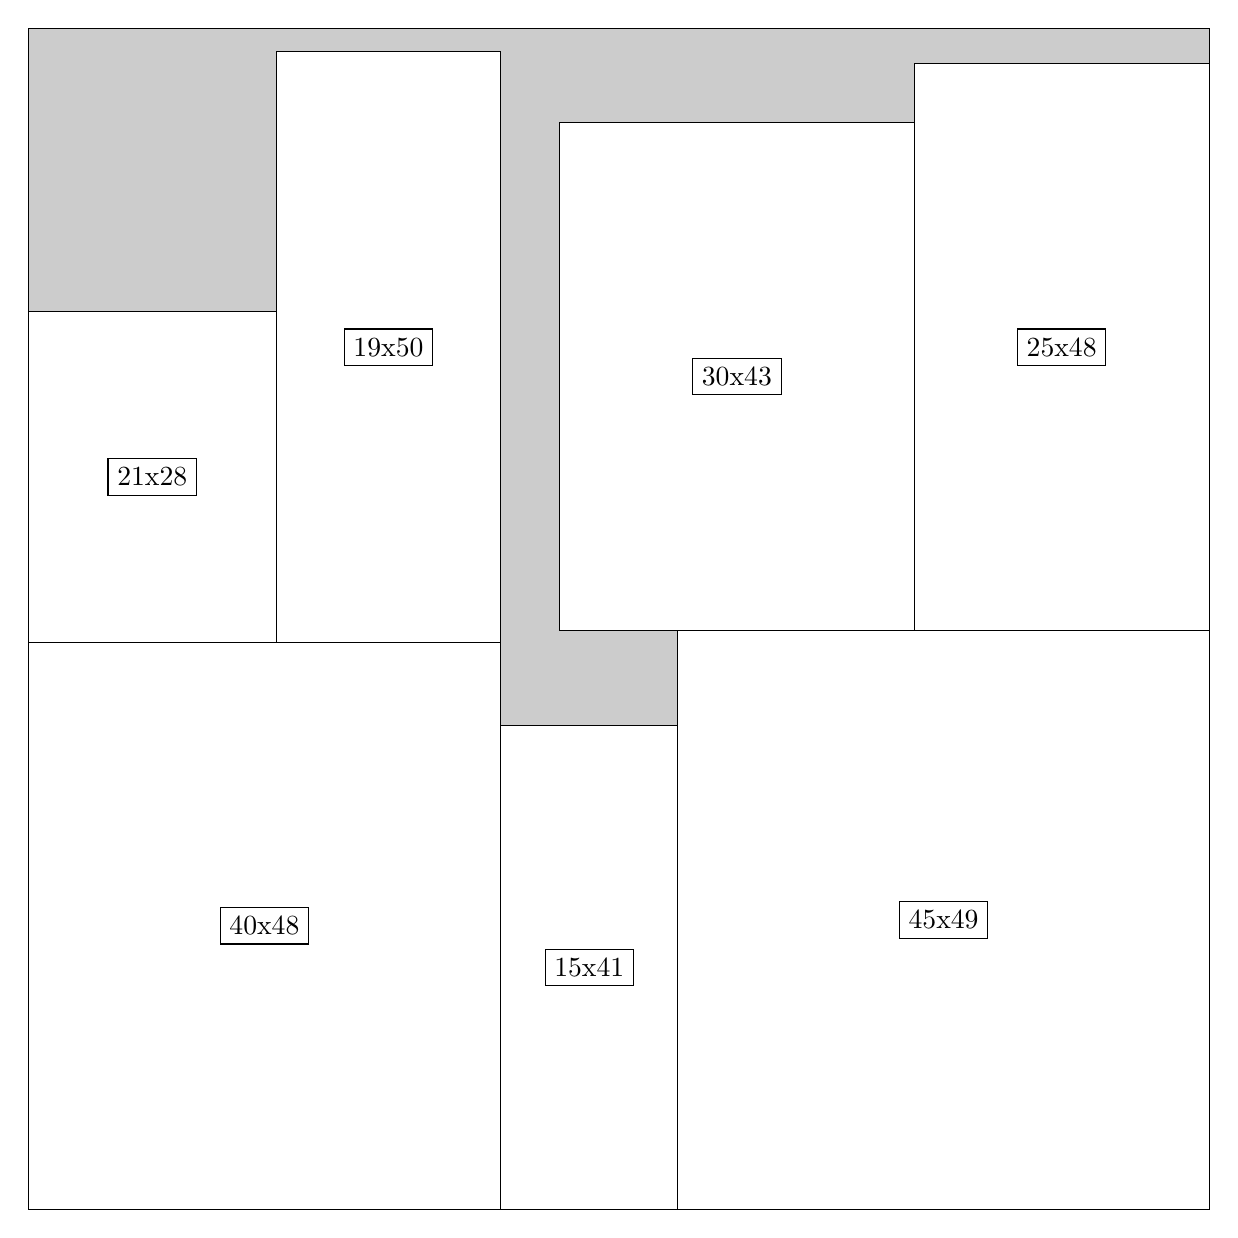
\begin{tikzpicture}[shorten >=1pt,scale=1.0,every node/.style={scale=1.0},->]
\tikzstyle{vertex}=[circle,fill=black!25,minimum size=14pt,inner sep=0pt]
\filldraw[fill=gray!40!white, draw=black] (0,0) rectangle (15.0,15.0);
\foreach \name/\x/\y/\w/\h in {45x49/8.25/0.0/6.75/7.35,15x41/6.0/0.0/2.25/6.1499999999999995,25x48/11.25/7.35/3.75/7.199999999999999,30x43/6.75/7.35/4.5/6.45,40x48/0.0/0.0/6.0/7.199999999999999,19x50/3.15/7.199999999999999/2.85/7.5,21x28/0.0/7.199999999999999/3.15/4.2}
\filldraw[fill=white!40!white, draw=black] (\x,\y) rectangle node[draw] (\name) {\name} ++(\w,\h);
\end{tikzpicture}


w =45 , h =49 , x =55 , y =0 , v =2205
\par
w =15 , h =41 , x =40 , y =0 , v =615
\par
w =25 , h =48 , x =75 , y =49 , v =1200
\par
w =30 , h =43 , x =45 , y =49 , v =1290
\par
w =40 , h =48 , x =0 , y =0 , v =1920
\par
w =19 , h =50 , x =21 , y =48 , v =950
\par
w =21 , h =28 , x =0 , y =48 , v =588
\par
\newpage


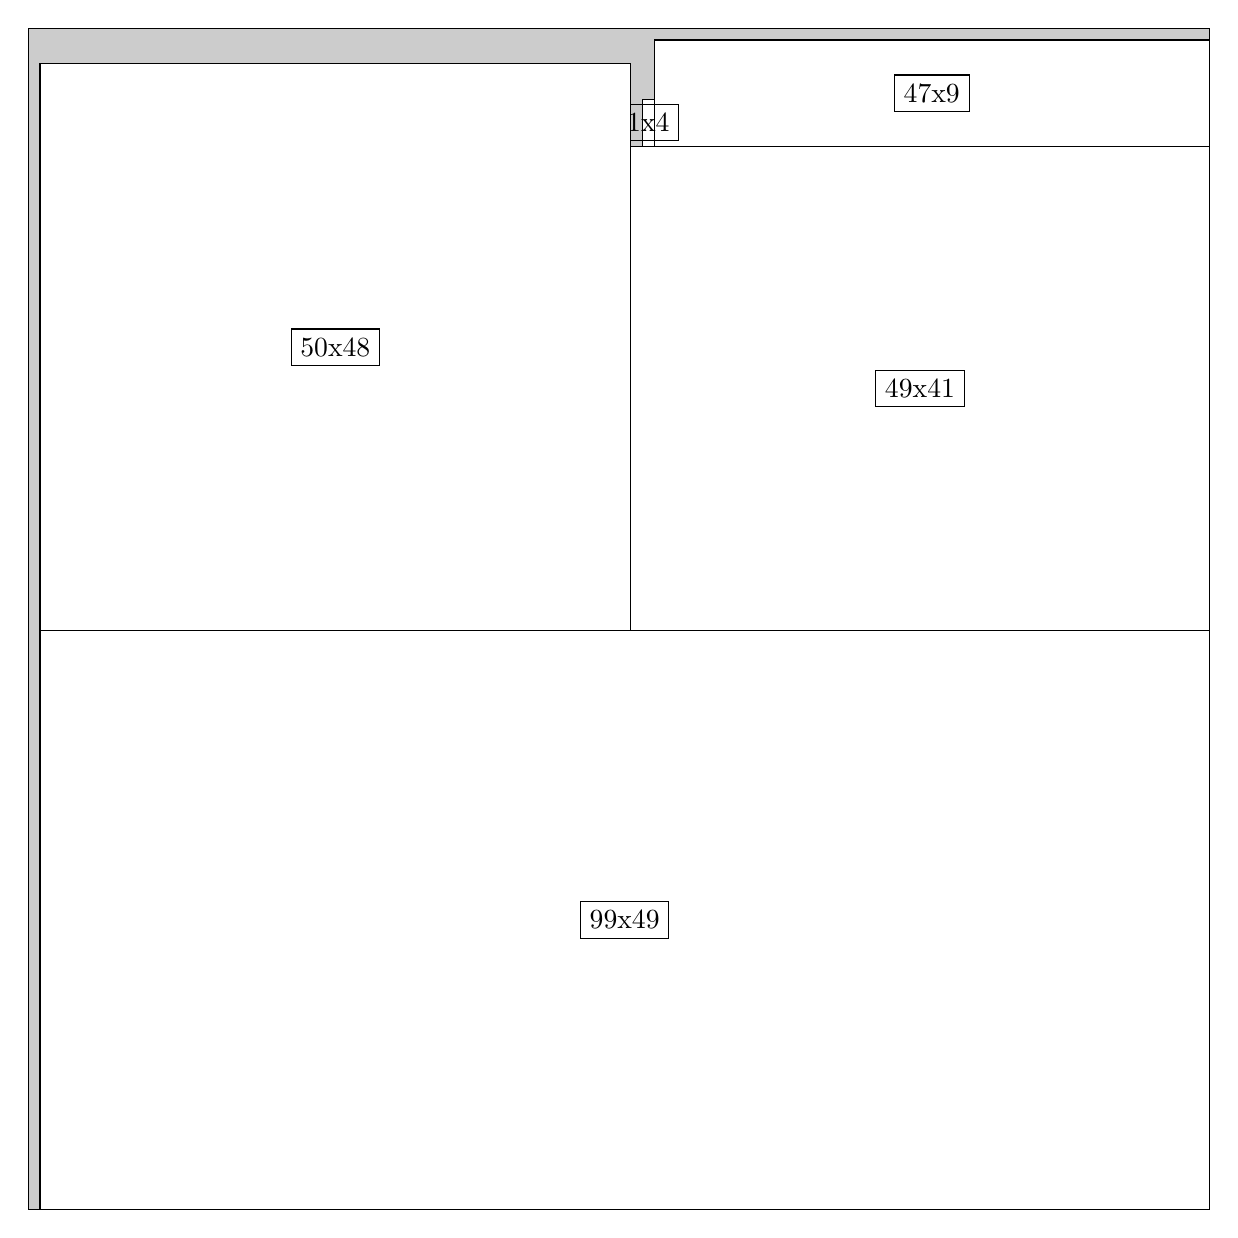
\begin{tikzpicture}[shorten >=1pt,scale=1.0,every node/.style={scale=1.0},->]
\tikzstyle{vertex}=[circle,fill=black!25,minimum size=14pt,inner sep=0pt]
\filldraw[fill=gray!40!white, draw=black] (0,0) rectangle (15.0,15.0);
\foreach \name/\x/\y/\w/\h in {99x49/0.15/0.0/14.85/7.35,49x41/7.6499999999999995/7.35/7.35/6.1499999999999995,47x9/7.949999999999999/13.5/7.05/1.3499999999999999,1x4/7.8/13.5/0.15/0.6,50x48/0.15/7.35/7.5/7.199999999999999}
\filldraw[fill=white!40!white, draw=black] (\x,\y) rectangle node[draw] (\name) {\name} ++(\w,\h);
\end{tikzpicture}


w =99 , h =49 , x =1 , y =0 , v =4851
\par
w =49 , h =41 , x =51 , y =49 , v =2009
\par
w =47 , h =9 , x =53 , y =90 , v =423
\par
w =1 , h =4 , x =52 , y =90 , v =4
\par
w =50 , h =48 , x =1 , y =49 , v =2400
\par
\newpage


\end{document}